\section{Auswertung}
\label{sec:Auswertung}
\subsection{Winkelrichtgröße und Eigenträgheitsmoment}
Die Winkelrichtgröße $D$ wird nach
\begin{equation*}
    D = \frac{F \cdot r}{\varphi}
\end{equation*} 
berechnet.
In Tab. \ref{tab:kraft} ist die gemessene Kraft $F$ für den Auslenkwinkel $\varphi$ und die resultierende Winkelrichtgrößte $D$ aufgeführt.
\begin{table}
    \centering
    \csvreader[tabular=c|c|c,
    head=false,
    table head= $\varphi/\si{\degree}$ & $F/\si{\newton}$ & $D/\si{\newton\metre}$\\
    \midrule,
    late after line= \\]
    {content/data/stange_D.csv}{1=\eins, 2=\zwei, 3=\drei}{$\num{\eins}$ & $\num{\zwei}$ & $\num{\drei}$}
    \caption{Die gemessene Kraft $F$ bei einem Auslenkwinkel $\varphi$ und die daraus resultierende Winkelrichtgröße $D$.}
    \label{tab:kraft}  
\end{table}
\FloatBarrier
Um den Mittelwert zu ermitteln wird die Formel
\begin{equation}
    \mu = \frac{1}{n} \sum_{i=1}^n x_i
\end{equation}
verwendet.
Wobei $x_i$ der $i$-te Wert bei $n$ Werten ist.
Um die Standardabweichung zu berechnen wird
\begin{equation}
    \sigma = \sqrt{\frac{1}{n-1} \sum_{i=1}^n (x_i - \mu)^2}
\end{equation}
verwendet.\\
Die Winkelrichtgrößte beträgt im Mittel
\begin{equation*}
    D = \SI{0.032(14)}{\newton\metre} .
\end{equation*}
\\
Um das Eigenträgheitsmoment zu Bestimmen, werden für verschiedene Abstände $a$ die Schwingungsdauer $T$ gemessen (siehe Tab. \ref{tab:gewichte}).
Die Masse der kleinen Gewichte beträgt jeweils $m_G = \SI{223,27}{\kg}$.
Sie haben die Form eines Zylinders mit Radius $r_G=\SI{1,75}{\centi\metre}$ und Höhe $h_G=\SI{3}{\centi\metre}$.
\begin{table}
    \centering
    \csvreader[tabular=c|c,
    head=false,
    table head= $a/\si{\centi\metre}$ & $T/\si{\hertz}$ \\
    \midrule,
    late after line= \\]
    {content/data/gewichte.csv}{1=\eins, 2=\zwei}{$\num{\eins}$ & $\num{\zwei}$}
    \caption{Die Schwingungsdauer $T$ bei variablem Abstand $r$ zur Drehachse.}
    \label{tab:gewichte}  
\end{table}
\FloatBarrier
Das Gesamtträgheitsmoment ergibt sich aus
\begin{equation*}
    I_{ges} = I_D + 2 I_G .
\end{equation*}
Mithilfe des Satz von Steiner folgt %ref
\begin{equation*}
    I_{ges} = I_D + 2 m_G \left ( \frac{r^2_G}{4} + \frac{h^2_G}{12} \right) + 2 m_G a^2 .
\end{equation*}
Eingesetzt in die Formel für die Schwingungsdauer $T$, ergibt sich %ref
\begin{equation}
    T^2 = \frac{8 \pi^2 m_G}{D} \cdot a^2 + \frac{4 \pi^2 I_D}{D} + \frac{8 \pi^2 m_G \left (\frac{r^2_G}{4} + \frac{h^2_G}{12} \right )}{D}
    \label{eqn:eigentraegheit}
\end{equation}
Nun wird eine lineare Ausgleichsrechnung durchgeführt.
Die Gleichung \ref{eqn:eigentraegheit} muss die Form
\begin{equation*}
    y = c \cdot x + b 
\end{equation*}
haben.
Daraus ergeben sich die Koeffizienten
\begin{equation*}
    c = \frac{8\pi^2m_G}{D}
\end{equation*}
und
\begin{equation}
    b = \frac{4 \pi^2 I_D}{D} + \frac{8 \pi^2 m_G \left (\frac{r^2_G}{4} + \frac{h^2_G}{12} \right )}{D}.
    \label{eqn:b}
\end{equation}
Hier gilt zudem $y = T^2$ und $x = a^2$.
Mithilfe des Python Plugin curvefit, folgt %ref
\begin{equation*}
    c = \SI{719(21)}{\frac{1}{\second^2 \metre^2}}
\end{equation*}
und
\begin{equation*}
    b = \SI{4.7(10)}{\hertz^2} .
\end{equation*}
Die lineare Ausgleichsrechnung ist in Abb. \ref{fig:ausgleich} dargestellt.
\begin{figure}
    \centering
    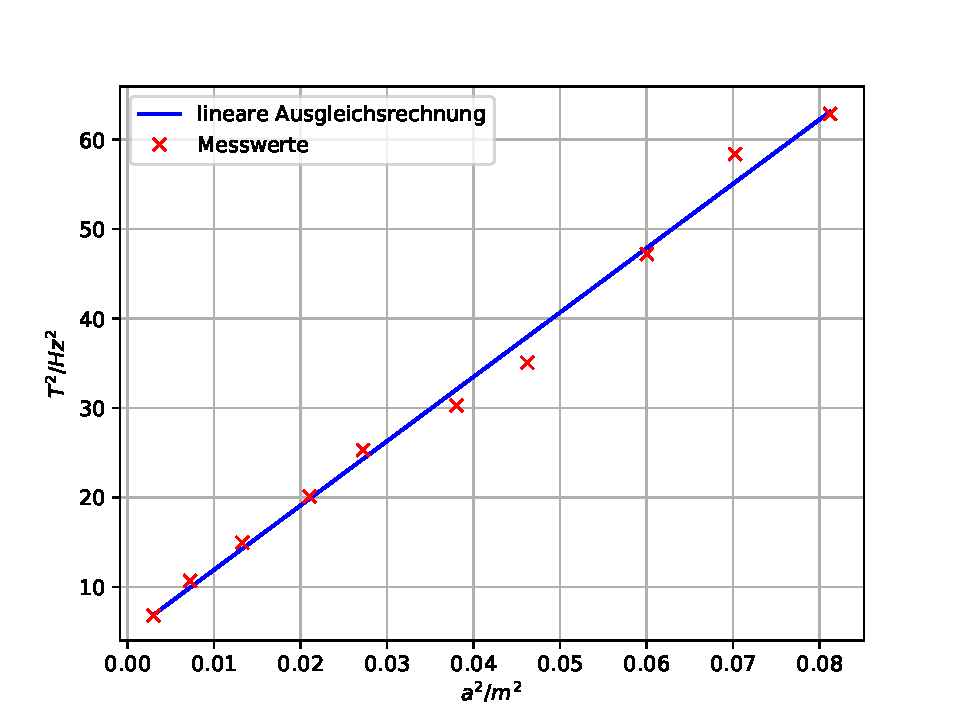
\includegraphics[width=\textwidth]{content/data/ausgleich.pdf}
    \caption{Lineare Ausgleichsrechnung um Eigenträgheitsmoment $I_\text{d}$ zu ermitteln.}
    \label{fig:ausgleich}
\end{figure}
Das gesuchte Eigenträgheitsmoment der Drillachse lässt sich nun mithilfe der Definition von $b$ (\autoref{eqn:b}) bestimmen:
\begin{equation*}
    I_D = \SI{0.0038(190)}{\metre^2\kg}
\end{equation*}

\FloatBarrier

\subsection{Trägheitsmoment eines großen Zylinders}
\begin{table}
    \centering
    \csvreader[tabular=c|c,
    head=false,
    table head= Messung & $T/\si{\second}$ \\
    \midrule,
    late after line= \\]
    {content/data/zylinder_gr.csv}{1=\eins, 2=\zwei}{$\num{\eins}$ & $\num{\zwei}$}
    \caption{Mehrfache Messung der Schwingungsdauer $T$ für den großen Zylinder.}
    \label{tab:zylinder_gr}  
\end{table}
\FloatBarrier

\subsection{Trägheitsmoment eines kleinen Zylinders}
\begin{table}
    \centering
    \csvreader[tabular=c|c,
    head=false,
    table head= Messung & $T/\si{\second}$ \\
    \midrule,
    late after line= \\]
    {content/data/zylinder_kl.csv}{1=\eins, 2=\zwei}{$\num{\eins}$ & $\num{\zwei}$}
    \caption{Mehrfache Messung der Schwingungsdauer $T$ für den kleinen Zylinder.}
    \label{tab:zylinder_kl}  
\end{table}
\FloatBarrier

\subsection{Trägheitsmomente der Modellpuppe}
\subsubsection{Position 1}
\begin{table}
    \centering
    \csvreader[tabular=c|c,
    head=false,
    table head= Messung & $T/\si{\second}$ \\
    \midrule,
    late after line= \\]
    {content/data/modellpuppe1.csv}{1=\eins, 2=\zwei}{$\num{\eins}$ & $\num{\zwei}$}
    \caption{Mehrfache Messung der Schwingungsdauer $T$ für die Modellpuppe in Position 1.}
    \label{tab:modellpuppe1}  
\end{table}
\FloatBarrier

\subsubsection{Position 2}
\begin{table}
    \centering
    \csvreader[tabular=c|c,
    head=false,
    table head= Messung & $T/\si{\second}$ \\
    \midrule,
    late after line= \\]
    {content/data/modellpuppe2.csv}{1=\eins, 2=\zwei}{$\num{\eins}$ & $\num{\zwei}$}
    \caption{Mehrfache Messung der Schwingungsdauer $T$ für die Modellpuppe in Position 2.}
    \label{tab:modellpuppe2}  
\end{table}
\FloatBarrier